% !TEX root = ..\main.tex
\section{Problem analysis} % Completar i corrector
% Should I add an introduction on how this problem could be interesting to solve to add it to the risk analysis at SIG?

Therefore, as stated with the research questions in section \ref{section:project-summary}, the primary goals of this project are:
Measuring the degree of source code dependency between a project and the libraries it uses, as well as measure the effort needed to replace these libraries.

\subsection{Measuring the degree of source code library dependency}
To the best of our knowledge, there are no papers about measuring the degree of dependency between two separate projects. However, it is true that the degree of dependency between two classes or modules of the same project has already been measured many times, using coupling metrics \cite{yu2011measurement}.

Therefore, we propose re-using the already existing coupling metrics, meant to measure the coupling between units of the \textit{same} project and adapt them to measure coupling \textit{between} projects.

\bigskip\noindent
According to Poshyvanyk and Marcus in \cite{poshyvanyk2006conceptual}, there are five main groups of coupling metrics:

\begin{itemize}
  \item \textbf{Structural coupling metrics:} Measured directly from static source code analysis. Largely studied by the related literature.

  \item \textbf{Dynamic coupling measures:} Measured using dynamic code analysis. "Introduced as the refinement to existing coupling measures due to gaps in addressing polymorphism, dynamic binding, and the presence of unused code by static structural coupling measures" \cite{poshyvanyk2006conceptual}.

  \item \textbf{Evolutionary and Logical coupling:} According to \cite{zimmermann2005mining}, evolutionary coupling can: "tell us which parts of the system are coupled by common changes or cochanges."

  \item \textbf{Coupling measures based on information entropy approach:} Coupling metrics based on the information-theory approach, such as the metrics proposed by Allen and Khoshgoftaar in \cite{allen1999measuring}.

  \item \textbf{Coupling metrics for specific types of software applications:} Specialized coupling metrics for certain types of projects, such as knowledge-based systems or aspect-oriented approach.
\end{itemize}

\bigskip\noindent
The last two categories are much more domain-specific. Moreover, the evolutionary coupling is not possible to be applied in our context since it is very likely that the separate projects are not going to evolve at the same time, given that they are not developed by the same team. Therefore, the research of this project, owing to the time limitation, is going to be centered on the structural metrics.

These metrics are going to be proposed as a first step to measure the degree of library dependency. These metrics can be extended and calculated more accurately by adding dynamic coupling metrics in case time permits or in future work.

\subsubsection{Structural coupling metrics}
There are many structural coupling metrics, each one measuring a different type of coupling from a different perspective, depending on the purpose for which the metrics are needed.
To decide which metrics can be applied to answer RQ1, we have compared all the metrics according to the papers from Briand et al. \cite{briand1999unified}, Poshyvanyk et al. \cite{poshyvanyk2006conceptual}, and Harrison et al. \cite{harrison1998coupling}. Based on the contents of these papers, we have created Table \ref{table:coupling-metrics}.

The empty cells in Table \ref{table:coupling-metrics} mean that the characteristic is unspecified for the metric in the papers. The \textit{Types of connections} assigned in Table \ref{table:coupling-metrics} as numbers correspond to the descriptions specified in Table \ref{table:types-connections}.

In the same way, the column \textit{Counting connections} has values from A to F, the meaning of which can be found in Table \ref{table:counting-connections}.
The content of both tables, more detailed descriptions, as well as a complete comparison between each type of connection and each way of counting connections, can be found in \cite{briand1999unified}.

\begin{table}[ht!]
    \begin{center}
    \begin{tabularx}{\textwidth}{|l|l|l|X|}
    \hline
    \# & Client Item & Server Item & Description \\
    \hline\hline
    1   & attribute \textit{a} of a class \textit{c} & class \textit{d}, d != c & class \textit{d} is the type of \textit{a} \\
    \hline
    2   & method \textit{m} of a class \textit{c} & class \textit{d}, d != c  & class \textit{d} is the type of a parameter of \textit{m}, or the return type of \textit{m} \\
    \hline
    3   & method \textit{m} of a class \textit{c} & class \textit{d}, d != c  & class \textit{d} is the type of a local variable of \textit{m} \\
    \hline
    4   & method \textit{m} of a class \textit{c} & class \textit{d}, d != c  & class \textit{d} is the type of a parameter of a method invoked by \textit{m} \\
    \hline
    5   & method \textit{m} of a class \textit{c} & \begin{tabular}[c]{@{}l@{}}attribute \textit{a} of a\\ class \textit{d}, d != c \end{tabular}  & \textit{m} references \textit{a} \\
    \hline
    6   & method \textit{m} of a class \textit{c} & \begin{tabular}[c]{@{}l@{}}method \textit{m'} of a\\ class \textit{d}, d != c \end{tabular} & \textit{m} invokes \textit{m'} \\
    \hline
    7   & class \textit{c} & class \textit{d}, d != c  & high-level relationships between classes, such as \textit{uses} or \textit{consists-of} \\
    \hline
    \end{tabularx}
    \end{center}
    \caption{Types of connections, obtained from \cite{briand1999unified}}
    \label{table:types-connections}
\end{table}

\begin{table}[htb!]
    \begin{center}
    \begin{tabularx}{\textwidth}{|l|l|X|}
    \hline
    \begin{tabular}[c]{@{}l@{}}Counting\\ connections\end{tabular} & Level & Description \\
    \hline\hline
    A   & \begin{tabular}[c]{@{}l@{}}Method or\\ attribute\end{tabular} & count individual connections  \\
     \hline
    B   & \begin{tabular}[c]{@{}l@{}}Method or\\ attribute\end{tabular} & count the number of distinct items at the other end of the connections  \\
     \hline
    C   & Class & add up the number of connections counted as in A) for each method or attribute of the class   \\
     \hline
    D   & Class & add up the number of connections counted as in B) for each method or attribute of the class   \\
     \hline
    E   & Class & count the number of distinct items at the end of connections starting from or ending in methods or attributes of the class    \\
     \hline
    F   & Class & for a class c, count the number of other classes to which there is at least  one connection  \\
    \hline
    \end{tabularx}
    \end{center}
    \caption{Counting connections, obtained from \cite{briand1999unified}}
    \label{table:counting-connections}
\end{table}

\begin{table}[p]
    \begin{center}
    \begin{tabular}{|l|l|l|l|l|l|l|}
    \hline
    \rot{Metric} & \rot{Inheritance} & \rot{Import or export} & \rot{Types of connection} & \rot{Domain of measure} & \rot{Counting connections  } & \rot{Indirect coupling} \\ \hline \hline
    CBO & both & both & 5, 6 & class & F & no \\
    CBO' & no & both & 5, 6 & class & F & no \\
    \hline
    $RFC_\alpha$ & both & import & 6 & class & E & depends \\
    RFC & both & import & 6 & class & E & no \\
    RFC' & both & import & 6 & class & E & yes \\
    \hline
    MPC & both & import & 6 & class & C & no \\
    \hline
    DAC & both & import & 1 & class & C & no \\
    DAC' & both & import & 1 & class & D & no \\
    \hline
    COF & no & both & 5, 6 & system & F & no \\
    \hline
    ICP & both & import & 6 & method, class, set & A, C & no \\
    IH-ICP & only & import & 6 & method, class, set & A, C & no \\
    NIH-ICP & no & import & 6 & method, class, set & A, C & no \\
    \hline
    IFCAIC & no & import & 1 & class &  & no \\
    ACAIC & only & import & 1 & class &  & no \\
    OCAIC & no & import & 1 & class &  & no \\
    FCAEC & no & export & 1 & class &  & no \\
    DCAEC & only & export & 1 & class &  & no \\
    OCAEC & no & export & 1 & class &  & no \\
    \hline
    IFCMIC & no & import & 2 & class & C & no \\
    ACMIC & only & import & 2 & class & C & no \\
    OCMIC & no & import & 2, 6 & class & C & no \\
    FCMEC & no & export &  & class & C & no \\
    DCMEC & only & export &  & class & C & no \\
    OCMEC & no & export &  & class & C & no \\
    \hline
    OMMIC & no & import &  & class & C & no \\
    IFMMIC & no & import & 6 & class & C & no \\
    AMMIC & only & import & 6 & class & C & no \\
    OMMEC & no & export & 6 & class & C & no \\
    FMMEC & no & export & 6 & class & C & no \\
    DMMEC & only & export & 6 & class & C & no \\
    \hline
    \end{tabular}
    \end{center}
    \caption{Coupling metrics comparison}
    \label{table:coupling-metrics}
\end{table}

\bigskip\noindent
The first metric of the table is CBO which stands for \textit{Coupling between Objects}. This metric counts the number of other classes to which it is coupled, the revised definition of the metric \cite{chidamber1994metrics}, includes inheritance. The revised version of the metric is CBO in Table \ref{table:coupling-metrics}, while the initial definition is CBO'.

The second group of metrics in the table are the \textit{Response for Class} metrics. This metric calculates the response set of a class. According to \cite{chidamber1994metrics}: \textit{"The response set of a class is a set of methods that can potentially be executed in response to a message received by an object of that class"}. The return set includes the methods called by the directs calls of the class, the methods that are called by transitivity. In \cite{briand199unified} it is considered that the inherited methods are included in this set since they can be executed to respond to a message received in the class. Based on this definition, there are three defined metrics, the first one being $RFC_\alpha$ \cite{churcher1995towards}. The $\alpha$ defines the number of nested levels that are considered in the calculcation of the metric. The other two metrics are special cases of this one: RFC is the case when $\alpha = 1$, and RFC' when $\alpha = \infty$.

The metric \textit{Message Passing Coupling} (MPC) \cite{li1993object} counts invocations of a class to methods of other classes, but only from new methods of the class. This means that the inherited methods are not accounted for. In \cite{briand1999unified}, the definition was changed to \textit{"the number of static invocations of methods not implemented in c by methods implemented in c"}. With the new definition, there is no more uncertainty about the overriden methods, or the calls to inherited methods.

Next, there is the group of \textit{Data Abstraction Coupling} (DAC) \cite{li1993object}. Due to the uncertainty in the original definition of this metric, in \cite{briand1999unified}, the metric is redefined as follows: \textit{"DAC is the number of not inherited attributes that have a class as their type. The number of the classes used as types for attributes is counted by DAC'"}.

The only metric which domain of measurement is the entire system is the \textit{Coupling Factor} (COF) \cite{abreu1995toward}. COF calculates the number of relations between classes of the system, which are not related through inheritance. The factor is normalized between 1 and 0 by dividing the number of relations by the maximum number of relations possible in the system. This way, it is possible to compare systems of different sizes.

The next group contains the metrics for \textit{Information-flow-based Coupling} (ICP). The original ICP metric counts \textit{"for method m of class c, the number of polymorphistically invoked methods of other classes, weighted by the number of parameters of the invoked method."}. From this description, the metric IH-ICP counts only inheritance-based coupling, whereas NIH-ICP counts coupling to those classes with which there is no inheritance relationship. The metric ICP is the sum of the previous two.

The rest of the metrics from Table \ref{table:coupling-metrics} are the suite of metrics defined by Briand et al. \cite{briand1997investigation}.To interpret the metrics suggested by Briand et al. \cite{briand1997investigation}  (from IFCAIC to DMMEC in Table \ref{table:coupling-metrics}), it is necessary to know they are named according to three variables: relationship, locus, and type. The name of each metric is composed in the following way, the initials of the relationship, the initials of the type of interaction, and the initials of the locus. These initials are described below.

\bigskip\noindent
There are three types of relationships, listed below, which can be used to determine the coupling of a class $c$. All the definitions have been obtained from \cite{briand1997investigation}.

\begin{itemize}
  \item Inheritance (A, D): Interactions from a class to its antecessors or descendents, depending on the locus.
  \item Friendship (F, IF): Extension for C++, interactions from class to all the  classes declared as friends or the classes that declare it their friend (inverse friends), depending on the locus.
  \item Other (O): interaction with classes that do not have an inheritance or friendship relationship.
\end{itemize}

\bigskip\noindent
The three different types of interaction descibed by Briand et al. \cite{briand1997investigation}, are the following:
\begin{itemize}
    \item Class-Atribute (CA): "There is a class-attribute (CA-)interaction from class c to class d, if an attribute of class c is of type class d."
    \item Class-Method (CM): "There is a class-method (CM-) interaction from class c to class d, if a newly defined method of class c has a parameter of type class d."
    \item Method-Method (MM): "There is a method-method (MM-)interaction from class c to class d, if a method implemented at class c statically invokes a method of class d (newly defined or overriding), or receives a pointer to such a method."
\end{itemize}

\bigskip\noindent
Finally, the two types of locus are:
\begin{itemize}
  \item Export from a class (EC): "Change flows away from a class", related to the descendants (D) and the friends (F).
  \item Import to a class (IC): "Change flows towards a class", related to the antecesors (A) and the inverse friends (IF).
\end{itemize}

\bigskip\noindent
Now that the metrics have been explained with the tables and the description of each of the metrics, we have to select the candidates to be used in the project.

First, the metric COF is calculating the factor of coupling of a system, and only within this system, therefore, it is not applicable in our case.

In Table \ref{table:coupling-metrics}, there are some metrics that incorporate inheritance to calculate coupling and some that do not.
Since we want to take into account each usage of the libraries in the projects, it is significant to measure both, inheritance and non-inheritance.
Therefore, the metrics CBO', IH-ICP and NIH-ICP will not be used for this project. The metrics by Briand et al. either only take the inheritance into account or not at all, but they can be combined to consider every type of dependency.

Furthermore, to take the \textit{transitive} dependencies into account, it is important to count transitive coupling as well.
In this manner, the metric $RFC_\alpha$ is truly interesting in this context.

In addition, the metric CBO does not consider multiple connections between the same two classes, only counts if there is at least one connection between the two classes. Therefore, since the goal in this project is to make a more fine grained evaluation of the coupling between the packages, this metric is not applicable.

Finally, the metrics that are being considered for this project, taking into account the criteria explained above, are the following:

\begin{itemize} % Revise definitions to see if it is necessary to discard more measures.
    \item $RFC_\alpha$
    \item MPC
    \item DAC, DAC'
    \item ICP
    \item Metrics by Briand et al. (only for one of the locus)
\end{itemize}

Finally, another option would be to consider the framework described in \cite{briand1999unified}.

\subsection{Measuring the effort needed to replace a library}
The typical way of estimating effort is by the means of models such as COCOMO II \cite{sharma2011analysis}, which calculate the effort to generate new code. However, for the second research question, it is necessary to find a way to calculate the effort to modify the existing code instead of developing new code. In \cite{kama2014cochcomo} and \cite{asl2013change}, Kama et al. present a tool for software change effort estimation, based on COCOMO II.

This tool, COCHCOMO, combines static and dynamic software analysis to calculate the effort to modify a part of the code. It takes the classes affected by the change into account, both directly and indirectly.

However, COCHCOMO is based on the requirements of the system. Given a change in a requirement, it estimates the effort needed to carry out the change, considering the classes affected by the requirement. The calculation process used in COCHCOMO could be adapted to base it on the replacement a library, instead of basing it on changes in the requirements.

It is also important to consider some new parameters added to this effort calculation. For instance, if the library is deemed to be replaced by another library (or multiple ones) or the features used from the library will be implemented in-house.

Plus, in \cite{kama2014cochcomo} the methodology contemplates the state of each of the classes (i.e. it is finished, in development or not started). It will be examined if this consideration is applicable in the case of this project or not.

\subsection{Proof-of-Concept}
To calculate the metrics as a proof-of-concept, it is necessary to create a dependency graph of the project. It has to be a call-level graph since we require a fine-grained analysis of the source code dependencies. Moreover, it has to represent the software ecosystem of the project considering the various versions of the libraries it uses. This way, it will avoid creating false-positives with library versions the project does not really use.

Most of the literature about modeling software ecosystems, use the nodes of the dependency graph to represent libraries or versions of these \cite{decan2017empirical, hejderup2015dependencies, kikas2017structure}. They are using a package-based approach. The problem with this approach is that, by using this node definition, it is not possible to determine which parts of the project are affected by a particular dependency. The same happens with measuring this dependency. Furthermore, a package-based graph could define transitive dependencies that do not really exist (see Figure \ref{fig:example-call-based} for an example).

\begin{figure}[ht!]
    \centering
    \fbox{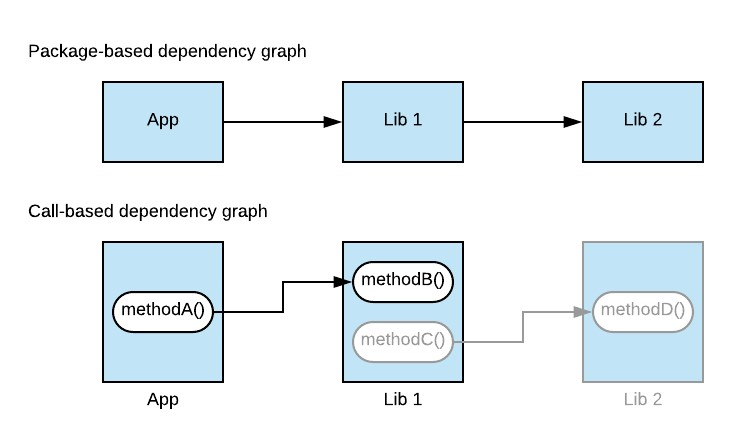
\includegraphics[width=0.8\textwidth]{img/example-call-based.jpg}}
    \caption{Comparison package-based and call-based dependency graphs.}
    \label{fig:example-call-based}
\end{figure}

\bigskip\noindent
Nevertheless, some papers do implement a call-based approach and therefore, could be used in this project.

Hejderup et al. in \cite{hejderup2018software}, propose the creation of a call-level dependency network, in which it can be determined which parts of the project depend on which library. Furthermore, this paper employs a different process to resolve dependencies, taking into account the evolution over time of the versions of the libraries on which the projects depend. Therefore, the analysis of the dependency degree and replacement effort would not be conducted exclusively per library, but also per version of each library.

 Hejderup et al. \cite{hejderup2018prazi}, propose an approach to create a call-based dependency network, PRÄZI. This approach, as the previous one, takes the versioning of the different libraries into account. It also considers that a certain project can depend on various versions of a library at the same time. In the paper, they implement it to create the dependency network of an entire software ecosystem (Crates.io). Nevertheless, this approach could be utilized to construct the network of a given project.

\subsection{Validation of the metrics}
Ultimately, the metrics used in this project will have to be validated. There is not a unique way to validate metrics which is globally accepted and used. Therefore, various approaches will be adopted to validate the metrics as holistically as possible.

In the paper \cite{srinivasan2014software}, Srinivasan et al. explain that there are two fundamental approaches for metric validation: \textit{theoretically} and \textit{empirically}. Therefore, to provide a check of validity that is as broad as possible, a mixture of these two approaches will be used during this project.

For the theoretical validity of the coupling metrics, we will validate that all of them fulfill the \textit{Mathematical Properties of Measures for Coupling}, described in \cite{srinivasan2014software}.

Furthermore, Meneely et al. \cite{meneely2013validating} describe a set of 47 validation criteria for metrics. The time limit of the project does not allow for a complete validation of all the metrics. Consequently, a sub-set of these criteria will be used to validate the metrics. This will be done for both the coupling and effort metrics.

The empirical validation of the metrics will be carried out by the means of case studies. For instance, the predicted effort corresponds to the real required effort, within a certain error window.
